%\documentclass{article}
%
%\usepackage{graphicx}
%\usepackage{caption}
%\usepackage{subcaption}
%\usepackage{pdflscape}
%
%
%
%\begin{document}
%\begin{landscape}
%	\begin{figure}
%		\centering
%		\begin{subfigure}{0.5\textwidth} % width of left subfigure
%			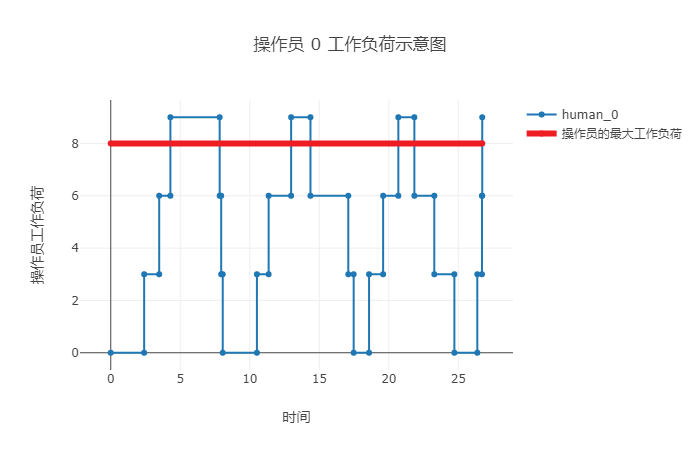
\includegraphics[width=\textwidth]{png/no_1.png}
%			\caption{RNC} % subcaption
%		\end{subfigure}
%		\vspace{1em} % here you can insert horizontal or vertical space
%		\begin{subfigure}{0.5\textwidth} % width of right subfigure
%			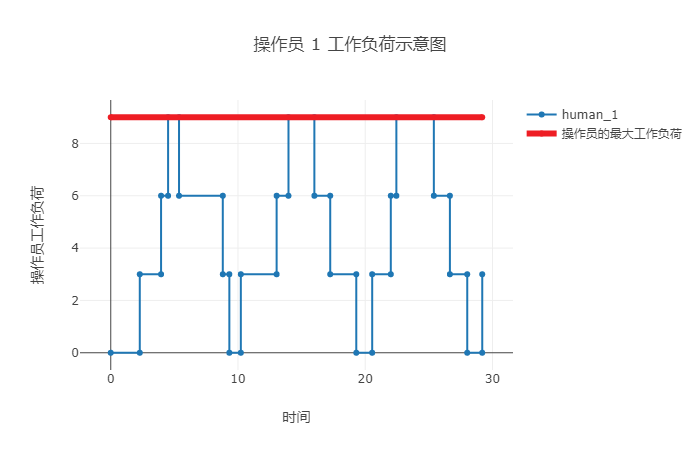
\includegraphics[width=\textwidth]{png/no_2.png}
%			\caption{DNC} % subcaption
%		\end{subfigure}	
%		\vspace{1em} % here you can insert horizontal or vertical space	
%		\begin{subfigure}{0.5\textwidth} % width of right subfigure
%		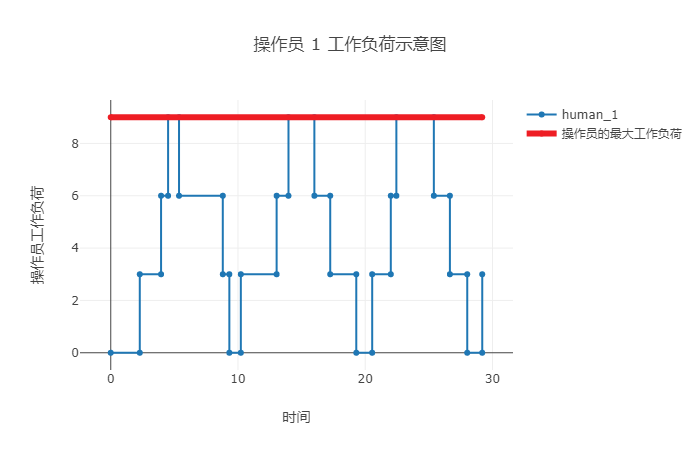
\includegraphics[width=\textwidth]{png/no_2.png}
%		\caption{DNC} % subcaption
%		\end{subfigure}
%
%		\centering
%		\vspace{1em} % here you can insert horizontal or vertical space	
%		\begin{subfigure}{0.5\textwidth} % width of right subfigure
%		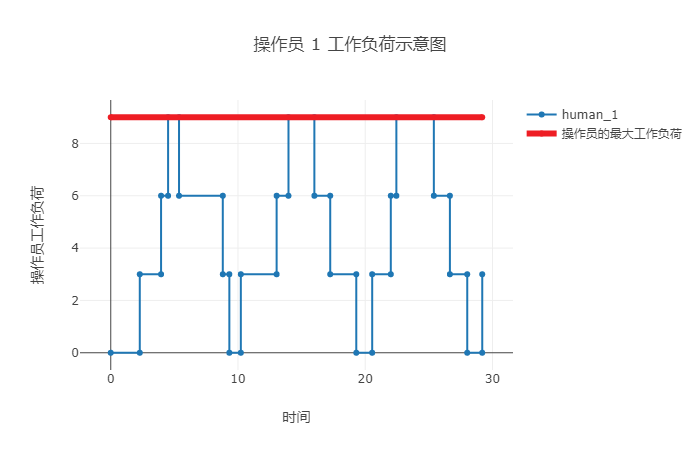
\includegraphics[width=\textwidth]{png/no_2.png}
%		\caption{DNC} % subcaption
%		\end{subfigure}
%	
%		\vspace{1em} % here you can insert horizontal or vertical space	
%		\begin{subfigure}{0.5\textwidth} % width of right subfigure
%		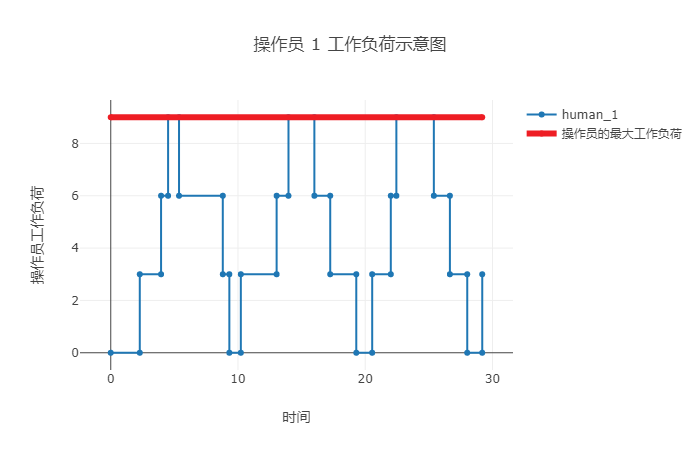
\includegraphics[width=\textwidth]{png/no_2.png}
%		\caption{DNC} % subcaption
%		\end{subfigure}
%	
%		\caption{Wordcloud of national conventions} % caption for whole figure
%	\end{figure}
%\end{landscape}	
%	
%\end{document}



\documentclass{article}
\usepackage[demo]{graphicx} % "demo" option just for this example
\usepackage{subcaption}
\usepackage{pdflscape}

\begin{document}
	\begin{landscape}
	\begin{figure}[t!] % "[t!]" placement specifier just for this example
		\centering				
		\begin{subfigure}{0.32\textwidth}
			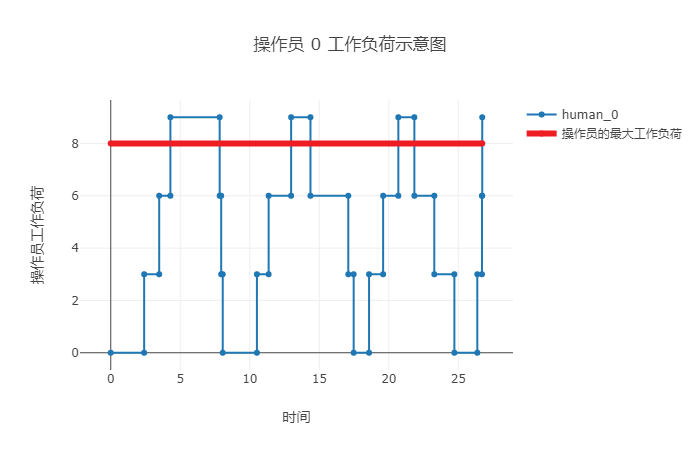
\includegraphics[width=\linewidth]{png/no_1.png}
			\caption{First subfigure} \label{fig:a}
		\end{subfigure}\hspace*{\fill}
		\begin{subfigure}{0.32\textwidth}
			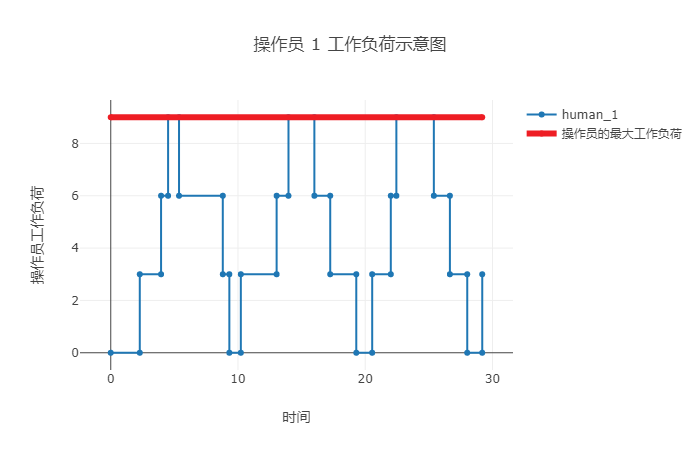
\includegraphics[width=\linewidth]{png/no_2.png}
			\caption{Second subfigure} \label{fig:b}
		\end{subfigure}\hspace*{\fill}		
		\begin{subfigure}{0.32\textwidth}
			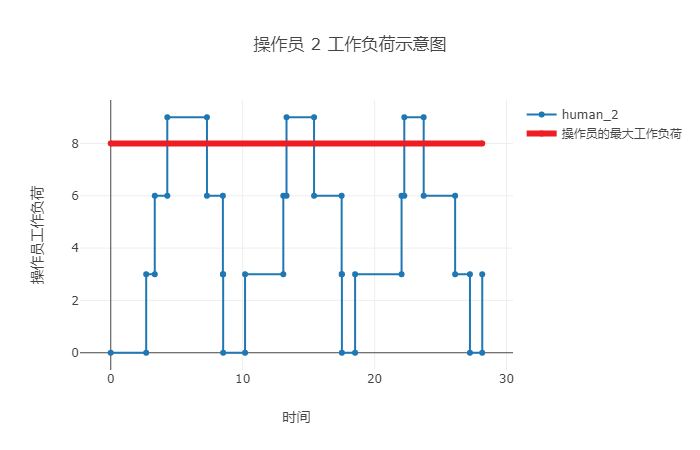
\includegraphics[width=\linewidth]{png/no_3}
			\caption{Third subfigure} \label{fig:c}
		\end{subfigure}\hspace*{\fill}
	 
%	  �˴��Ŀո񲻿���ȡ��	
		\medskip		
		\begin{subfigure}{0.32\textwidth}
			\centering			
			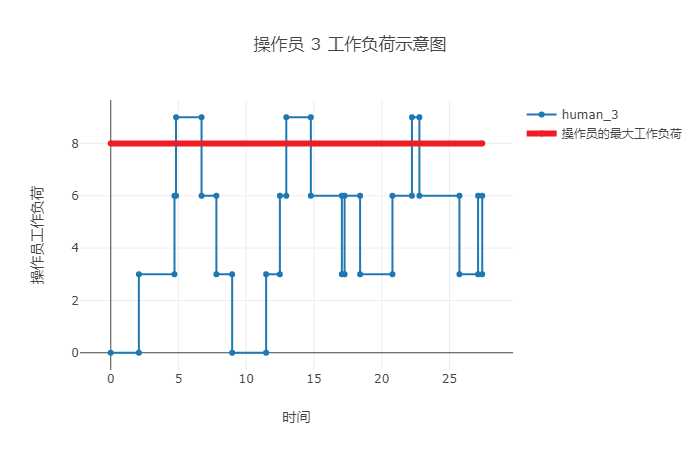
\includegraphics[width=\linewidth]{png/no_4}
			\caption{Fifth subfigure} \label{fig:e}
		\end{subfigure}\hspace*{\fill}
		\begin{subfigure}{0.32\textwidth}
			\centering						
			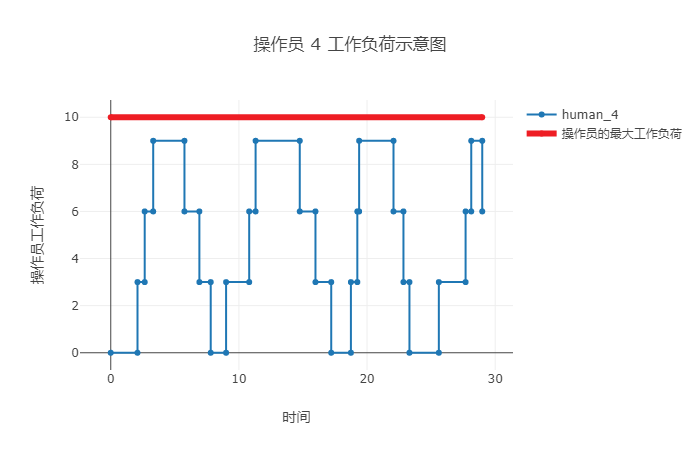
\includegraphics[width=\linewidth]{png/no_5}
			\caption{Sixth subfigure} \label{fig:f}
		\end{subfigure}\hspace*{\fill}		
		\caption{My complicated figure} \label{fig:1}
	\end{figure}
	\end{landscape}
	A cross-reference to Figure~\ref{fig:1}, and a cross-reference to Subfigure~\ref{fig:e}.
\end{document}

